\section{Planning}
\label{sec:planning}
\subsection{Method}
%\todo[inline, author=Michael]{Either we should shorten this section or add a more brief description (to get an overview) in the beginning (aka. right here). This could be the nice enumerate in the conclusion(sec. 2.3).}
%\todo[inline, author=Lukas]{Maybe just have the full code example once and then refer to lines or similar?...}

The robot is modelled as a point robot by letting the configuration space be the freespace padded with obstacles,
with padding length equal to the robot dynamics radius.
This padding is obtained using the brushfire algorithm with a Norm-2 potential function (rounded corners),
and then simply applying a threshold in the map for the padding.


\subsubsection{Offline processing}

As all information about the map (excluding the location of the cups) is known to the robot prior to movement,
it was chosen to carry out much of the planning offline.
A short overview of the approach is given below. 

\begin{enumerate}
\item Generate map of brushfire values, \(M_{B,0}\), from original image.
\item Generate a new image with closed doors, considered obstacles, using \(M_{B,0}\).
\item Generate a map of brushfire values, \(M_{B,D}\) from the image with closed doors.
\item Generate a set of coordinates, \(S_{D}\), from \(M_{B,D}\),
such that the brushfire values of the coordinates in \(S_{D}\) are odd multiples of the robot scanner radius.
\item Generate a set of coordinates, \(S_{L}\) (initialized to \(S_{D}\)), by merging coordinates with local brushfire value maxima
in \(M_{B,D}\), with \(S_{D}\), selecting only coordinates that are not within one robot scanner radius
of any coordinate already in the set.
\item Generate a set of coordinates, \(S_{M}\) (initialized to \(S_{L}\)), of all the coordinates that need to be scanned
to guarantee detection of all cups, by adding from the freespace all remaining coordinates
that are not within one robot scanner radius of any coordinate already in \(S_{M}\).
\end{enumerate}



\begin{figure}[ht]
\centering
  \begin{subfigure}[t]{0.3\textwidth}
    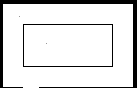
\includegraphics[width = \textwidth]{graphics/sq/dist}
    \caption{Brushfire based coverage}
    \label{sqdist}
  \end{subfigure}
  \begin{subfigure}[t]{0.3\textwidth}
    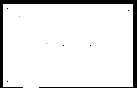
\includegraphics[width = \textwidth]{graphics/sq/top}
    \caption{Points that were not covered by wall distance}
    \label{sqtop}
  \end{subfigure}  
  \begin{subfigure}[t]{0.3\textwidth}
    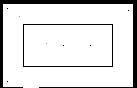
\includegraphics[width = \textwidth]{graphics/sq/list}
    \caption{List formed by merging the two list}
    \label{sqlist}
  \end{subfigure}
\caption{Offline planning}
\label{offline_steps}
\end{figure}

To detect all cups, the entire map must be scanned.
In other words, there is a minimum number of coordinates for the robot to cover.
Several sets of coordinates satisfy the criterion that the entire map would be scanned if they were each visited.
Of course, setting this set to hold all freespace coordinates would not make for very good off-line planning.
Therefore, it was chosen to use a map, \(M_{B,0}\), generated by the brushfire algorithm,
mapping a brushfire value to each coordinate, to generate the set of coordinates.

We denote all coordinates with brushfire values equal to odd multiples of the robot scanner radius \(S_{B}\).
These coordinates is shown in figure \ref{sqdist}.
\(S_{B}\) consists of lines of points, with all points on a given line having the same distance to the walls.
If the robot always moves to the nearest point in \(S_{B}\),
it would follow these lines and cover most of the map.
However, large rooms (with large doorways and local lines inside) would be entered multiple times,
including the long and relatively narrow hallways.
This is neither very pedagogical or practical, considering the interruptions created
from the need to open doors, and the extra length that would be traveled
in hallways, compared to if each room was visited only once.
Therefore, it was chosen to create a different map, \(M_{B,D}\), of brushfire values from the idea
that all doors are closed and function as obstacles.
Selecting coordinates from \(M_{B,D}\) according to the same criterion as the one used for \(M_{B,0}\),
a different set, \(S_{D}\), of coordinates to visit is obtained.
\(S_{D}\) is similiar to \(S_{B}\), but with an important difference:
There are no lines going through doorways.
With this set of coordinates, if the robot always moves to the closest point,
it will still stick to the lines while, this time, staying inside the rooms until all the local lines
have been visited.

\(S_{D}\) is not the complete set of coordinates the robot needs to visit.
Some local brushfire value maxima in the centres of rooms would need to be scanned,
but are not in \(S_{D}\), because they are not odd multiples of the robot scanner radius.
Of course, these local maxima are easy to find, using \(M_{B,D}\), and the coordinates
are merged with \(S_{D}\), creating a new set, \(S_{L}\).
The coordinates are shown in figure \ref{sqtop}.
The coordinates are merged into \(S_{L}\) one at a time, and are only chosen if no coordinates
of \(S_{L}\) are (already) within one robot scanner radius.
The final list is shown in figure \ref{sqlist}.

\(S_{L}\) consists of almost all points that need to be scanned in order to detect all cups.
Only a few coordinates of freespace remain to be scanned. These are merged with \(S_{L}\)
into a new set, \(S_{M}\).
They are added much in the same way as the local brushfire value maxima:
The entire freespace is searched for coordinates that are not close to any coordinates in \(S_{M}\),
and these are added to \(S_{M}\) until no more coordinates remain to be scanned.
Thus, \(S_{M}\) is the complete set of coordinates that need to be scanned to detect all cups.

The robot will need to visit the offloading stations when its cup capacity is reached, and it should
reach these stations quickly. Since the offloading stations are stationary, a map, \(M_{OL}\) is created,
holding values generated by Dijkstra's Shortest Path with Weighted Costs algorithm, using a Norm-2 potential function
for the wave propagation from the offloading stations.

\subsubsection{Online processing}

Each time the robot moves one step (from one coordinate to another),
it needs to do three things: Scan, pick up cups within reach, decide whether or not to move to the offloading stations.
% suggestion... I only suggest because it will shorten program run time and it is unnecessary to scan areas twice.
%>>> Since list \(S_{M}\) covers the entire map there is no need to scan when the robot is not standing on a coordinate that is a member of \(S_{M}\).
% ===
The coordinates that need to be scanned are all in the set \(S_{M}\).
% <<<
Thus, to ensure the entire map is scanned, the robot only needs to visit all coordinates of \(S_{M}\).
The scan range is shown as the red circle in figure \ref{sqroomscan0}.
Optimally, the route taken through these coordinates is as short as possible,
making this a case of the Traveling Salesman Problem.
To keep the number of computations for calculating the route low, it was chosen to find a suboptimal solution to the problem.
For each coordinate visited in \(S_{M}\), the nearest neighbour strategy is used to select the next coordinate in \(S_{M}\) to visit.
This movement is simple to code, as illustrated by below pseudo-code:

\begin{verbatim}
while( S_M is not empty ){
   c = Nearest coordinate in S_M;
   s = Shortest path to c;
   for( each coordinate i in s ){
      Move robot to i;
      Scan with robot scanner centered at i.
      Remove i from S_M;
   }
}
\end{verbatim}

The above pseudo-code handles the scanning of the entire map.
The picking up of cups within reach can easily be added after the scan,
but what about the cups that are found by the scanner, yet are unreachable?
To keep the code simple, these cups are handled indirectly: They (or configuration space coordinates close to them) are added to \(S_{M}\):
Figure \ref{sqroomscan0} shows a cup that is unreachable. 
By keeping to the nearest neighbour the robot will move to the left. 
In figure \ref{sqroom_scan1} the robot is in a position where the cup is reachable and the coordinate is removed from \(S_{M}\). 
Following this logic the map is covered as shown in figure \ref{sqcoverage}. 

\begin{verbatim}
while( S_M is not empty ){
   c = Nearest coordinate in S_M;
   s = Shortest path to c;
   for( each coordinate i in s ){
      Move robot to i;
      Scan with robot scanner centered at i;
      for( each cup coordinate k in the circle ){
         if( k is reachable ){
            Pick up the cup at k;
         }
         else{
            Add k's nearest configuration space coordinate to S_M;
         }
      }
      Remove i from S_M;
   }
}
\end{verbatim}

Now, all that's left is handling the situation where the robot reaches its cup capacity.
It was chosen to make the necessary modification to the above pseudo-code as simple as possible:
If the robot reaches its cup capacity, it returns to the nearest offloading station coordinate,
taking the shortest path available, scanning for cups on the way. When the offloading station is reached,
the robot returns to the nearest-neighbour strategy (it does not return the way it came).
The modification, concluding the robot movement logic, is indicated in the pseudo-code below.

\begin{verbatim}
while( S_M is not empty ){
   c = Nearest coordinate in S_M;
   s = Shortest path to c;
   for( each coordinate i in s ){
      Move robot to i;
      Scan with robot scanner centered at i;
      for( each cup coordinate k in the circle ){
         if( k is reachable ){
            Pick up the cup at k;
            if( cup capacity reached ){
               z = Shortest path to offloading station (using M_OL);
               for( each coordinate j in z ){
                  Move robot to j;
                  Remove j from S_M;
                  Scan with robot scanner centered at j;
                  for( each cup coordinate g in the circle ){
                     Add g's nearest configuration space coordinate to S_M;
                  }
               }
            }
         }
         else{
            Add k's nearest configuration space coordinate to S_M;
         }
      }
      Remove i from S_M;
   }
}
\end{verbatim}

The selection of the nearest neighbour is performed using the wavefront algorithm, propagating
a wave around the robot until a coordinate in \(S_{M}\) is found.
The robot movement is shown in figure \ref{sqpath}.

\begin{figure}[ht]
\centering
  \begin{subfigure}[t]{0.3\textwidth}
    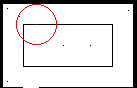
\includegraphics[width = \textwidth]{graphics/sq/room_scan0}
    \caption{Cup is out of reach, Cup is added to list}
    \label{sqroomscan0}
  \end{subfigure}
  \begin{subfigure}[t]{0.3\textwidth}
    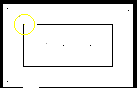
\includegraphics[width = \textwidth]{graphics/sq/room_scan1}
    \caption{Cups inside pickup range is removed}
    \label{sqroom_scan1}
  \end{subfigure}
    
  \begin{subfigure}[t]{0.3\textwidth}
    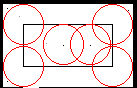
\includegraphics[width = \textwidth]{graphics/sq/coverage}
    \caption{Coverage in critical areas}
    \label{sqcoverage}
  \end{subfigure}
  \begin{subfigure}[t]{0.3\textwidth}
    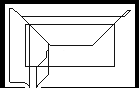
\includegraphics[width = \textwidth]{graphics/sq/path}
    \caption{The traveled path}
    \label{sqpath}
  \end{subfigure}
  \caption{Online planning}
  \label{online_planning}
\end{figure}
